\documentclass[../Tesi.tex]{subfiles}


\begin{document}
\section{Progettazione}
	\subsection{Architettura ad alto livello}
		\begin{figure}[!h]
			\centering
			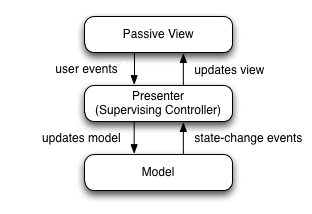
\includegraphics[scale=0.6]{images/mvp}
				\caption{Rappresentazione pattern MVP}
			\label{fig:StrutturaMVP}
		\end{figure}

		L'architettura dell'applicazione segue il pattern architetturale Model-View-Presenter, utilizzato insieme alla dependency injection. Tale scelte, unite ad un uso diffuso di interfacce permettono di ridurre il grado di accoppiamento tra le parti che l'applicazione in modo tale da aumentarne il più possibile l'estensibilità.

		\paragraph*{Model}
		Il model rappresenta i dati che vengono trattati all'interno dell'applicazione. Le classe appartenenti al model rappresentano:
		\begin{itemize}
			\item i dati che vengono salvati in modo persistente nel database presente nel dispositivo in cui è installata l'applicazione;
			\item gli statement che devono essere inviati ad un LRS;
			\item gli oggetti che vengono scambiati tra JavaScript e Android per il tracciamento delle esperienze di un utente;
			\item oggetti che permettono l'accesso a tali dati.
		\end{itemize}
		Nell'applicativo è rappresentato dal package omonimo.

		\paragraph*{Presenter}
		Il presenter si occupa di recuperare i dati del model e passarli alla view per essere mostrati. Esso si occupa inoltre di gestire le richieste della view in seguito ad una interazione con un utente. \\ Nell'applicativo è rappresentato dal package omonimo.

		\paragraph*{View}
		La view si occupa della dell'interfaccia grafica dell'applicazione e di notificare al presenter le interazioni dell'utente, che ha il compito di elaborare. \\ Nell'applicativo è rappresentato dal package omonimo.
	
	\subsection{Persistenza dei dati}
		\subsubsection{Il database locale}
		L'applicazione si appoggia su di un database creato utilizzando la libreria Realm per il salvataggio dei dati relativi agli utenti, ai contenuti e alla loro fruizione in un database locale. In tale database vengono salvati i dati relativi ai contenuti xAPI che devono essere visualizzati la prima volta che l'applicazione viene avviata, mentre i dati relativi all'utente vengono salvati quando viene effettuato un login alla registrazione. I dati di fruizione, invece, all'interazione di un utente con un contenuto.
			
			\paragraph{Diagramma ER}

			\begin{figure} [H]
				\centering
				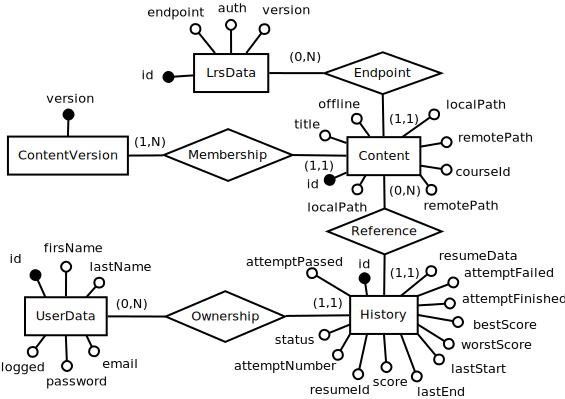
\includegraphics[scale=0.9]{images/er/RealmDB}
					\caption{Diagramma ER del database locale}
			\end{figure}

			\paragraph{Descrizione delle relazioni}
			\subparagraph*{Content}
			Relazione che contiene le informazioni dei contenuti xAPI che devono essere gestiti dall'applicazione. Attributi:
			\begin{itemize}
				\item \textbf{id}: chiave primaria, intero;
				\item \textbf{title}: stringa, rappresenta un titolo associato al contenuto;
				\item \textbf{remotePath}: stringa, rappresenta l'URL a cui è possibile recuperare il contenuto;
				\item \textbf{localPath}: stringa, rappresenta il percorso locale al dispositivo a cui è possibile recuperare il contenuto, se questo è disponibile offline;
				\item \textbf{offline}: boolean, indica se il contenuto è disponibile per la riproduzione offine oppure no;
				\item \textbf{courseId}: stringa, rappresenta l'identificativo utilizzato dal LRS per distinguere un contenuto;
				\item \textbf{lrsDataId}: intero, chiave esterna verso la relazione LrsData.
			\end{itemize}

				\subparagraph*{ContentVersion}
				Relazione che serve per specificare la versione dei contenuti trattati dall'appliaczione. Attributi:
				\begin{itemize}
					\item \textbf{version}: chiave primaria, stringa, rappresenta la versione dei contenuti.
				\end{itemize}

				\subparagraph*{LrsData}
				Relazione che contiene le informazioni riguardanti un LRS a cui inviare i dati di fruizione dei contenuti di un certo utente. Attributi:
				\begin{itemize}
					\item \textbf{id}: chiave primaria, intero;
					\item \textbf{endpoint}: stringa, rappresenta l'URL a cui inviare gli statement in formato xAPI;
					\item \textbf{auth}: stringa, rappresenta metodo e dati per l'accesso al LRS;
					\item \textbf{version}: stringa, rappresenta la versione di statement xAPI accettata dal LRS.
				\end{itemize}

				\subparagraph*{History}
				Relazione che contiene i dati di fruizione di ogni contenuto per gli utenti che hanno utilizzato l'applicazione su di un determinato dispositivo. Attributi:
				\begin{itemize}
					\item \textbf{id}: chiave primaria, intero;
					\item \textbf{resumeId}: stringa, identificativo utilizzato dalla componente che si occupa della riproduzione dei contenuti xAPI per l'accesso ai dati per riprendere un contenuto da dove lo si aveva interrotto all'ultima fruizione;
					\item \textbf{resumeData}: stringa, dati per riprendere un contenuto da dove lo si aveva interrotto all'ultima fruizione;
					\item \textbf{status}: intero, reppresenta lo stato in cui si trova un contenuto per un certo utente. Può rappresentare che un utente non ha mai acceduto ad un certo contenuto, che vi ha acceduto ma il contenuto non è stato fruito fino alla fine oppure che un utente ha superato o meno un certo contenuto;
					\item \textbf{score}: double, rappresenta l'ultimo punteggio ottenuto da un utente per un certo contenuto;
					\item \textbf{bestScore}: double, rappresenta il miglior punteggio ottenuto da un utente per un certo contenuto;
					\item \textbf{worstScore}: double, rappresenta il peggior punteggio ottenuto da un utente per un certo contenuto;
					\item \textbf{lastStart}: long, timestamp in millisecondi dell'ultima volta che un utente ha iniziato un certo contenuto;
					\item \textbf{lastStart}: long, timestamp in millisecondi dell'ultima volta che un utente ha terminato un certo contenuto;
					\item \textbf{attemptNumber}: intero, rappresenta il numero di volte che un utente ha iniziato un certo contenuto;
					\item \textbf{attemptFinished}: intero, rappresenta il numero di volte che un utente ha terminato un certo contenuto;
					\item \textbf{attemptPassed}: intero, rappresenta il numero di volte che un utente ha superato un certo contenuto;
					\item \textbf{attemptFailed}: intero, rappresenta il numero di volte che un utente non ha superato un certo contenuto;
					\item \textbf{contentId}: intero, chiave esterna verso la relazione Content. Rappresenta il contenuto a cui fanno riferimento i dati;
					\item \textbf{userId}: intero, chiave esterna verso la relazione UserData. Rappresenta l'utente a cui fanno riferimento i dati.
				\end{itemize}

				\subparagraph*{UserData}
				Relazione che contiene le informazioni degli utenti che hanno utilizzato l'applicazione su di un determinato dispositivo. Attributi:
				\begin{itemize}
					\item \textbf{id}: chiave primaria, intero;
					\item \textbf{logged}: boolean, indica se un utente è loggato in quel dispositivo o meno;
					\item \textbf{email}: stringa, rappresenta l'email di un utente;
					\item \textbf{password}: stringa, rappresenta la password di un utente;
					\item \textbf{firstName}: stringa, rappresenta il nome di un utente;
					\item \textbf{lastName}: stringa, rappresenta il cognome di un utente.
				\end{itemize}

			\paragraph{Descrizione delle associazioni}
				\subparagraph*{Membership}
				Associazione che unisce ogni contenuto alla sua versione.\\
				\textbf{Molteplicità}:(1,N) ogni versione può essere associato a più contenuti, ogni contenuto può avere un'unica versione.

				\subparagraph*{Endpoint}
				Associazione che unisce ogni contenuto al LRS a cui devono essere inviati i dati di fruizione.\\
				\textbf{Molteplicità}:(1,N) ogni LrsData può essere associato a più contenuti, ogni contenuto si riferisce ad un unico LrsData.

				\subparagraph*{Reference}
				Associazione che unisce ogni contenuto ai dati di fruizione per un certo utente.\\
				\textbf{Molteplicità}:(1,N) ogni contenuto può essere associato a più History, ogni History può essere associata ad un solo contenuto.

				\subparagraph*{Ownership}
				Associazione che unisce ogni utente ai dati di fruizione di un certo contenuto.\\
				\textbf{Molteplicità}:(1,N) ogni utente può essere associato a più History, ogni History può appartenere ad un unico utente.

			\subsubsection{Persistenza degli statement}
			Gli statement creati dall'applicazione per registrare i dati di fruizione dei contenuti xAPI sono salvati temporaneamente all'interno di un database SQLite, completamente gestito dalla libreria TinCanAndroid-Offline. Quando l'applicazione registra che è disponibile una connessione internet si occupa di inviare tali statement ad un LRS. Anche l'invio è gestito dalla libreria TinCanAndroid-Offline, che provvede, nel caso in cui non vi siano errori, ad eliminare dal database locale tutti gli statement inviati. Ad ogni avvio l'applicativo ha il compito di interrogare LRS a cui sono stati inviati i dati di fruizione al fine di verificare se vi siano dati che non sono presenti in locale: se presenti il database locale viene aggiornato. Poichè LRS utilizzato è Learning Locker, il quale utilizza come DBMS MongoDB, le richieste per recuperare dati dal LRS saranno delle query MongoDB e i risultati di tali richieste saranno in formato JSON.

			\subsubsection{Autenticazione e registrazione}
			L'autenticazione e la registrazione all'applicazione avvengono mediante delle richieste HTTP a due URL specificati nel file di configurazione dell'applicativo. Tale scelta è stata fatta per permettere di cambiare agevolmente tali indirizzi senza dover modificare il codice. \\In fase di sviluppo sono stati creati anche due script PHP ed un database per gli utenti dell'applicazione. Tali script si occupano rispettivamente del login e della registrazione, interrogando il database degli utenti e restituendo il risultato della richiesta.

\end{document}